
%%%%%%%%%%%%%%%%%%%%%%%%%%%%%%%%%%%%%%%%%
% Programming/Coding Assignment
% LaTeX Template
%
% This template has been downloaded from:
% http://www.latextemplates.com
%
% Original author:
% Ted Pavlic (http://www.tedpavlic.com)
%
% Note:
% The \lipsum[#] commands throughout this template generate dummy text
% to fill the template out. These commands should all be removed when 
% writing assignment content.
%
% This template uses a Perl script as an example snippet of code, most other
% languages are also usable. Configure them in the "CODE INCLUSION 
% CONFIGURATION" section.
%
%%%%%%%%%%%%%%%%%%%%%%%%%%%%%%%%%%%%%%%%%

%----------------------------------------------------------------------------------------
%	PACKAGES AND OTHER DOCUMENT CONFIGURATIONS
%----------------------------------------------------------------------------------------



\documentclass{article}

\usepackage{fancyhdr} % Required for custom headers
\usepackage{lastpage} % Required to determine the last page for the footer
\usepackage{extramarks} % Required for headers and footers
\usepackage[usenames,dvipsnames]{color} % Required for custom colors
\usepackage{graphicx} % Required to insert images
\usepackage{listings} % Required for insertion of code
\usepackage{courier} % Required for the courier font
\usepackage{lipsum} % Used for inserting dummy 'Lorem ipsum' text into the template
\usepackage{setspace}
\usepackage{color}
\usepackage{comment}
\usepackage{caption}
\usepackage[T1]{fontenc}
\usepackage{hyperref}
%\usepackage{natbib}
\usepackage{underscore}
\usepackage{subfigure}
\usepackage{fixltx2e}

\hypersetup{
    colorlinks=true,
    linkcolor=blue,
    filecolor=magenta,      
    urlcolor=cyan,
    breaklinks=true
}

\usepackage[]{algorithm2e}
\usepackage{pdfpages}
\usepackage{tikz}




%For python inclusion (http://widerin.org/blog/syntax-highlighting-for-python-scripts-in-latex-documents)
\definecolor{Code}{rgb}{0,0,0}
\definecolor{Decorators}{rgb}{0.5,0.5,0.5}
\definecolor{Numbers}{rgb}{0.5,0,0}
\definecolor{MatchingBrackets}{rgb}{0.25,0.5,0.5}
\definecolor{Keywords}{rgb}{0,0,1}
\definecolor{self}{rgb}{0,0,0}
\definecolor{Strings}{rgb}{0,0.63,0}
\definecolor{Comments}{rgb}{0,0.63,1}
\definecolor{Backquotes}{rgb}{0,0,0}
\definecolor{Classname}{rgb}{0,0,0}
\definecolor{FunctionName}{rgb}{0,0,0}
\definecolor{Operators}{rgb}{0,0,0}
\definecolor{Background}{rgb}{0.98,0.98,0.98}

% Margins
\topmargin=-0.45in
\evensidemargin=0in
\oddsidemargin=0in
\textwidth=6.5in
\textheight=9.0in
\headsep=0.25in

\linespread{1.1} % Line spacing

% Set up the header and footer
\pagestyle{fancy}
\lhead{\hmwkAuthorName} % Top left header
\chead{\hmwkClass\ (\hmwkClassInstructor\ \hmwkClassTime): \hmwkTitle} % Top center head
\chead{\hmwkClass\ (\hmwkClassInstructor): \hmwkTitle} % Top center head
\rhead{\firstxmark} % Top right header
\lfoot{\lastxmark} % Bottom left footer
\cfoot{} % Bottom center footer
\rfoot{Page\ \thepage\ of\ \protect\pageref{LastPage}} % Bottom right footer
\renewcommand\headrulewidth{0.4pt} % Size of the header rule
\renewcommand\footrulewidth{0.4pt} % Size of the footer rule

\setlength\parindent{0pt} % Removes all indentation from paragraphs

%----------------------------------------------------------------------------------------
%	CODE INCLUSION CONFIGURATION
%----------------------------------------------------------------------------------------

\definecolor{MyDarkGreen}{rgb}{0.0,0.4,0.0} % This is the color used for comments
\lstloadlanguages{Perl} % Load Perl syntax for listings, for a list of other languages supported see: ftp://ftp.tex.ac.uk/tex-archive/macros/latex/contrib/listings/listings.pdf
\lstset{language=Perl, % Use Perl in this example
        frame=single, % Single frame around code
        basicstyle=\small\ttfamily, % Use small true type font
        keywordstyle=[1]\color{Blue}\bf, % Perl functions bold and blue
        keywordstyle=[2]\color{Purple}, % Perl function arguments purple
        keywordstyle=[3]\color{Blue}\underbar, % Custom functions underlined and blue
        identifierstyle=, % Nothing special about identifiers                                         
        commentstyle=\usefont{T1}{pcr}{m}{sl}\color{MyDarkGreen}\small, % Comments small dark green courier font
        stringstyle=\color{Purple}, % Strings are purple
        showstringspaces=false, % Don't put marks in string spaces
        tabsize=5, % 5 spaces per tab
        %
        % Put standard Perl functions not included in the default language here
        morekeywords={rand},
        %
        % Put Perl function parameters here
        morekeywords=[2]{on, off, interp},
        %
        % Put user defined functions here
        morekeywords=[3]{test},
       	%
        morecomment=[l][\color{Blue}]{...}, % Line continuation (...) like blue comment
        numbers=left, % Line numbers on left
        firstnumber=1, % Line numbers start with line 1
        numberstyle=\tiny\color{Blue}, % Line numbers are blue and small
        stepnumber=5 % Line numbers go in steps of 5
}

% Creates a new command to include a perl script, the first parameter is the filename of the script (without .pl), the second parameter is the caption
\newcommand{\perlscript}[2]{
\begin{itemize}
\item[]\lstinputlisting[caption=#2,label=#1]{#1.pl}
\end{itemize}
}


%----------------------------------------------------------------------------------------
%	DOCUMENT STRUCTURE COMMANDS
%	Skip this unless you know what you're doing
%----------------------------------------------------------------------------------------

% Header and footer for when a page split occurs within a problem environment
\newcommand{\enterProblemHeader}[1]{
\nobreak\extramarks{#1}{#1 continued on next page\ldots}\nobreak
\nobreak\extramarks{#1 (continued)}{#1 continued on next page\ldots}\nobreak
}

% Header and footer for when a page split occurs between problem environments
\newcommand{\exitProblemHeader}[1]{
\nobreak\extramarks{#1 (continued)}{#1 continued on next page\ldots}\nobreak
\nobreak\extramarks{#1}{}\nobreak
}

\setcounter{secnumdepth}{0} % Removes default section numbers
\newcounter{homeworkProblemCounter} % Creates a counter to keep track of the number of problems

\newcommand{\homeworkProblemName}{}
\newenvironment{homeworkProblem}[1][Problem \arabic{homeworkProblemCounter}]{ % Makes a new environment called homeworkProblem which takes 1 argument (custom name) but the default is "Problem #"
\stepcounter{homeworkProblemCounter} % Increase counter for number of problems
\renewcommand{\homeworkProblemName}{#1} % Assign \homeworkProblemName the name of the problem
\section{\homeworkProblemName} % Make a section in the document with the custom problem count
\enterProblemHeader{\homeworkProblemName} % Header and footer within the environment
}{
\exitProblemHeader{\homeworkProblemName} % Header and footer after the environment
}

\newcommand{\problemAnswer}[1]{ % Defines the problem answer command with the content as the only argument
\noindent\framebox[\columnwidth][c]{\begin{minipage}{0.98\columnwidth}#1\end{minipage}} % Makes the box around the problem answer and puts the content inside
}

\newcommand{\homeworkSectionName}{}
\newenvironment{homeworkSection}[1]{ % New environment for sections within homework problems, takes 1 argument - the name of the section
\renewcommand{\homeworkSectionName}{#1} % Assign \homeworkSectionName to the name of the section from the environment argument
\subsection{\homeworkSectionName} % Make a subsection with the custom name of the subsection
\enterProblemHeader{\homeworkProblemName\ [\homeworkSectionName]} % Header and footer within the environment
}{
\enterProblemHeader{\homeworkProblemName} % Header and footer after the environment
}

%----------------------------------------------------------------------------------------
%	NAME AND CLASS SECTION
%----------------------------------------------------------------------------------------

\newcommand{\hmwkTitle}{Assignment\ \#6 } % Assignment title
%\newcommand{\hmwkDueDate}{Monday,\ January\ 1,\ 2012} % Due date
\newcommand{\hmwkClass}{Web Science} % Course/class
%\newcommand{\hmwkClassTime}{10:30am} % Class/lecture time
\newcommand{\hmwkClassInstructor}{Alexander Nwala} % Teacher/lecturer
\newcommand{\hmwkAuthorName}{Puneeth Bikkasandra} % Your name

%----------------------------------------------------------------------------------------
%	TITLE PAGE
%----------------------------------------------------------------------------------------

\title{
\vspace{2in}
\textmd{\textbf{\hmwkClass:\ \hmwkTitle}}\\
%\normalsize\vspace{0.1in}\small{Due\ on\ \hmwkDueDate}\\
%\vspace{0.1in}\large{\textit{\hmwkClassInstructor\ \hmwkClassTime}}
\vspace{0.1in}\large{\textit{\hmwkClassInstructor}}
\vspace{3in}
}

\author{\textbf{\hmwkAuthorName}}
\date{Sunday, March 31, 2018} % Insert date here if you want it to appear below your name

%----------------------------------------------------------------------------------------

\begin{document}

\maketitle
\newpage



%----------------------------------------------------------------------------------------
%	TABLE OF CONTENTS
%----------------------------------------------------------------------------------------

%\setcounter{tocdepth}{1} % Uncomment this line if you don't want subsections listed in the ToC

\newpage
\tableofcontents
\newpage

%----------------------------------------------------------------------------------------
%	PROBLEM 1
%----------------------------------------------------------------------------------------

% To have just one problem per page, simply put a \clearpage after each problem

\begin{homeworkProblem}

The goal of this project is to use the basic recommendation principles we have learned for user-collected data. 
You will modify the code given to you which performs movie recommendations from the MovieLense data sets.
(https://github.com/arthur-e/Programming-Collective-Intelligence/blob/master/chapter2/recommendations.py) 
The MovieLense data sets were collected by the GroupLens Research Project at the University of Minnesota 
during the seven-month period from September 19th, 1997 through April 22nd, 1998.  \\
We are using the  "100k dataset", available for download from: \\
http://grouplens.org/datasets/movielens/100k/\\

There are three files which we will use:

\begin{enumerate}
\item\textbf{}  u.data: 100,000 ratings by 943 users on 1,682 movies. Each user has rated at least 20 movies. 
Users and items are numbered consecutively from 1. The data is randomly ordered. 
\item\textbf{}  u.item: Information about the 1,682 movies.
\item\textbf{}  u.user: Demographic information about the users.
 \end{enumerate}
 
Find 3 users who are closest to you in terms of age,  gender, and occupation.  For each of those 3 users:

\begin{enumerate}
\item\textbf{} what are their top 3 favorite films?
\item\textbf{} bottom 3 least favorite films?
 \end{enumerate}
 
Based on the movie values in those 6 tables (3 users X (favorite + least)), choose a user that you feel is most like you. 
Feel free to note any outliers (e.g., "I mostly identify with user 123, except I did not like ``Ghost'' at all").  

This user is the "substitute you".
  
 \newpage
 
%\problemAnswer{

 \textbf{SOLUTION :}\\
 
I have solved the problem as described in the below steps :
  \begin{enumerate}
  \item\textbf{} I have set the parameters, 'Age', 'Gender' and 'Occupation' as '27', 'M', 'Student' respectively.
  \item\textbf{} Identified the matching users from \textbf{u.user} dataset, i received 6 such users.
  \item\textbf{} Chose 3 users with following Ids : \textbf{758, 429, 104}						      
 \end{enumerate}
%}
  
\begin{lstlisting}[language=Python, caption=approximateUser.py]
from operator import itemgetter

matchingUsers = []
myAge = 27
myOccupation = 'student'
myGender = 'M' 
userMoviesDict = {}
userMovieRatingDict = {}
finalTopThree = {}
finalBottomThree = {}
userMovieRatingsList = []
movieRatingsList = []
matches = ''
bottomCount = 0
topCount = 0
listSize = 0

with open('users.txt', 'r') as f1:
    for line in f1:
        userId,age,gender,occupation,zipcode = line.split('|')
        # if((int(age) < int(myAge) and int(age) > int((myAge - 3))) and (gender == myGender) and (occupation == myOccupation)):
        if((int(age) == myAge) and (gender == myGender) and (occupation == myOccupation)):	
        	matchingUsers.append(userId)

print matchingUsers        	

with open('data.txt', 'r') as f2:
    for line in f2:
        userId,movieId,rating,mseconds = line.split('	')
        if(userId in matchingUsers):
        	if(userId in userMoviesDict):
        		userMoviesDict[userId] = userMoviesDict[userId] + ":" + movieId + "|" + rating 
        	else :
        		userMoviesDict[userId] = movieId + "|" + rating 

print('--------')
for key, value in userMoviesDict.items():
	# print(key,userMoviesDict[key])
	userMovieRatingsList = userMoviesDict[key].split(":")
	for movieRating in userMovieRatingsList:
		movie,rating = movieRating.split("|")
		userMovieRatingDict[movie] = rating
		# print(movie,rating)

	sortedRatings = sorted(userMovieRatingDict.items(), key=lambda value: value[1])
	# print("Length :",len(sortedRatings))
	bottomCount = 0
	topCount = 0
	listSize = 0
	bottomMovieData = ""
	topMovieData = ""
	for data in sortedRatings:
		listSize = listSize + 1
		if(bottomCount < 3):
			if(bottomMovieData == ""):
				bottomMovieData = str(data)
			else :
				bottomMovieData = bottomMovieData + ":" + str(data)
			bottomCount = bottomCount + 1
		if(listSize > len(sortedRatings) - 3):
			if(topMovieData == ""):
				topMovieData = str(data)
			else :
				topMovieData = topMovieData + ":" + str(data)

	finalBottomThree[key] = bottomMovieData
	finalTopThree[key] = topMovieData
	print('--------------')	
	print(finalTopThree)
	print(finalBottomThree)
	print('\n')
	
print "User" + "  " + "Movie Title" + "  " + "Rating"
print "----" + "  " + "-----------" + "  " + "------"
for key, value in finalTopThree.items():	
	movieTuple = finalTopThree[key].split(":")
	for movie in movieTuple:
		movieId,rating = str(movie).split(",")
		movieId = movieId.replace("(","").replace("'","")
		with open('item.txt', 'r') as file:
			for line in file:
				mid,movieTitle = line.split("|")[0:2]
				if(mid == movieId):
					print key,"  "+ movieTitle+"  "+rating.replace(")","").replace("'","")

print('\n')

print "User" + "  " + "Movie Title" + "  " + "Rating"
print "----" + "  " + "-----------" + "  " + "------"
for key, value in finalBottomThree.items():	
	movieTuple = finalBottomThree[key].split(":")
	for movie in movieTuple:
		movieId,rating = str(movie).split(",")
		movieId = movieId.replace("(","").replace("'","")
		with open('item.txt', 'r') as file:
			for line in file:
				mid,movieTitle = line.split("|")[0:2]
				if(mid == movieId):
					print key,"  "+ movieTitle+"  "+rating.replace(")","").replace("'","")
\end{lstlisting}

The above code, will generate top 3 favorite and bottom 3 least favorite movies from the selected 3 users.

\begin{figure}[h]
  \centering
    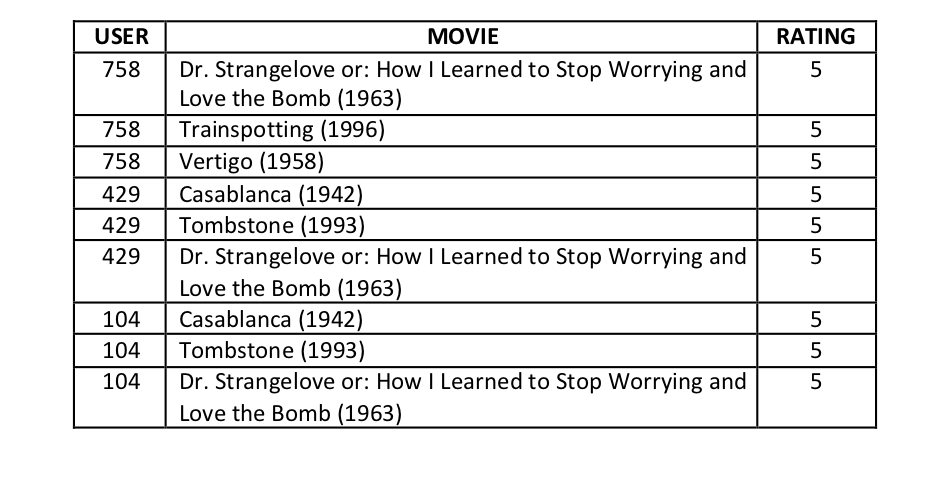
\includegraphics[width=0.6\textwidth]{top3}
     \caption{Top 3 Favorite Movies}
	\end{figure}

\begin{figure}[h]
  \centering
    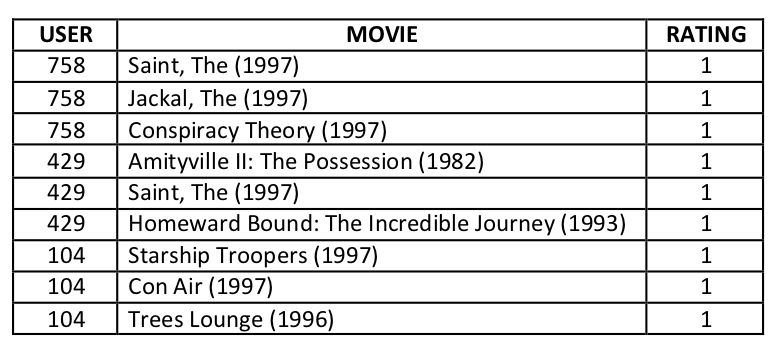
\includegraphics[width=0.6\textwidth]{bottom3}
     \caption{Bottom 3 Favorite Movies}
	\end{figure}
	
\end{homeworkProblem}
\clearpage
\newpage

%----------------------------------------------------------------------------------------
%   PROBLEM 2
%----------------------------------------------------------------------------------------

\begin{homeworkProblem}
2.  Which 5 users are most correlated to the substitute you? Which 5 users are least correlated (i.e., negative correlation)?\\
%\problemAnswer{

 \textbf{SOLUTION}\\
 
To solve this problem, i have used the code from the text \textbf{Programming Collective Intelligence}
I have chosen user \textbf{429} as '\textbf{Substitute Me} and pass the preferences of the 'Substitute Me'
to the \textbf{sim_pearson} function, to determine the nearest 5 users.

 		      
\begin{lstlisting}[language=Python, caption=correlation.py]
import csv
import math
import operator
import string
from collections import Counter
from math import sqrt

def sim_distance(prefs, p1, p2):
	'''
	Returns a distance-based similarity score for person1 and person2.
	'''

	# Get the list of shared_items
	si = {}
	for item in prefs[p1]:
		if item in prefs[p2]:
			si[item] = 1
	# If they have no ratings in common, return 0
	if len(si) == 0:
		return 0
	# Add up the squares of all the differences
	sum_of_squares = sum([pow(prefs[p1][item] - prefs[p2][item], 2) for item in
						 prefs[p1] if item in prefs[p2]])
	return 1 / (1 + sqrt(sum_of_squares))


def sim_pearson(prefs, p1, p2):
	'''
	Returns the Pearson correlation coefficient for p1 and p2.
	'''

	# Get the list of mutually rated items
	si = {}
	for item in prefs[p1]:
		if item in prefs[p2]:
			si[item] = 1
	# If they are no ratings in common, return 0
	if len(si) == 0:
		return 0
	# Sum calculations
	n = len(si)
	# Sums of all the preferences
	sum1 = sum([prefs[p1][it] for it in si])
	sum2 = sum([prefs[p2][it] for it in si])
	# Sums of the squares
	sum1Sq = sum([pow(prefs[p1][it], 2) for it in si])
	sum2Sq = sum([pow(prefs[p2][it], 2) for it in si])
	# Sum of the products
	pSum = sum([prefs[p1][it] * prefs[p2][it] for it in si])
	# Calculate r (Pearson score)
	num = pSum - sum1 * sum2 / n
	den = sqrt((sum1Sq - pow(sum1, 2) / n) * (sum2Sq - pow(sum2, 2) / n))
	if den == 0:
		return 0
	r = num / den
	return r


def topMatches(
	prefs,
	person,
	n=5,
	similarity=sim_pearson,
):
	'''
	Returns the best matches for person from the prefs dictionary. 
	Number of results and similarity function are optional params.
	'''

	scores = [(similarity(prefs, person, other), other) for other in prefs
			  if other != person]
	scores.sort()
	scores.reverse()
	return scores[0:n]


def getRecommendations(prefs, person, similarity=sim_pearson):
	'''
	Gets recommendations for a person by using a weighted average
	of every other user's rankings
	'''

	totals = {}
	simSums = {}
	for other in prefs:
	# Don't compare me to myself
		if other == person:
			continue
		sim = similarity(prefs, person, other)
		# Ignore scores of zero or lower
		if sim <= 0:
			continue
		for item in prefs[other]:
			# Only score movies I haven't seen yet
			if item not in prefs[person] or prefs[person][item] == 0:
				# Similarity * Score
				totals.setdefault(item, 0)
				# The final score is calculated by multiplying each item by the
				#   similarity and adding these products together
				totals[item] += prefs[other][item] * sim
				# Sum of similarities
				simSums.setdefault(item, 0)
				simSums[item] += sim
	# Create the normalized list
	rankings = [(total / simSums[item], item) for (item, total) in
				totals.items()]
	# Return the sorted list
	rankings.sort()
	rankings.reverse()
	return rankings


def transformPrefs(prefs):
	'''
	Transform the recommendations into a mapping where persons are described
	with interest scores for a given title e.g. {title: person} instead of
	{person: title}.
	'''

	result = {}
	for person in prefs:
		for item in prefs[person]:
			result.setdefault(item, {})
			# Flip item and person
			result[item][person] = prefs[person][item]
	return result


def calculateSimilarItems(prefs, n=10):
	'''
	Create a dictionary of items showing which other items they are
	most similar to.
	'''

	result = {}
	# Invert the preference matrix to be item-centric
	itemPrefs = transformPrefs(prefs)
	c = 0
	for item in itemPrefs:
		# Status updates for large datasets
		c += 1
		if c % 100 == 0:
			print('%d / %d' % (c, len(itemPrefs)))
		# Find the most similar items to this one
		scores = topMatches(itemPrefs, item, n=n, similarity=sim_distance)
		result[item] = scores
	return result


def getRecommendedItems(prefs, itemMatch, user):
	userRatings = prefs[user]
	scores = {}
	totalSim = {}
	# Loop over items rated by this user
	for (item, rating) in userRatings.items():
		# Loop over items similar to this one
		for (similarity, item2) in itemMatch[item]:
			# Ignore if this user has already rated this item
			if item2 in userRatings:
				continue
			# Weighted sum of rating times similarity
			scores.setdefault(item2, 0)
			scores[item2] += similarity * rating
			# Sum of all the similarities
			totalSim.setdefault(item2, 0)
			totalSim[item2] += similarity
	# Divide each total score by total weighting to get an average
	rankings = [(score / totalSim[item], item) for (item, score) in
				scores.items()]
	# Return the rankings from highest to lowest
	rankings.sort()
	rankings.reverse()
	return rankings

 

def loadMovieLens():
  # Get movie titles
	movies = {}
	for line in open('item.txt'):
		(id, title) = line.split('|')[0:2]
		movies[id] = title
  # Load data
	prefs = {}
	for line in open('data.txt'):
		(user, movieid, rating, ts) = line.split('\t')
		prefs.setdefault(user, {})
		prefs[user][movies[movieid]] = float(rating)
	return prefs

prefs = loadMovieLens()

with open('users.txt') as tsv:
	for line in csv.reader(tsv, delimiter="|"):
	   p2 = (line[0])
	   p1 = '429' 
	   r = sim_pearson(prefs, p1, p2) 
	   with open('corrlate.csv','a') as f:
			writer=csv.writer(f)
			writer.writerow([r,p2,p1])
	  	   
\end{lstlisting} 
%}

\newpage
The above code will generate \textbf{corrlate.csv}, which gives the correlation of all the users in comparison with 'Substitute Me' i.e., user \textbf{429}

	
\begin{figure}[h]
  \centering
    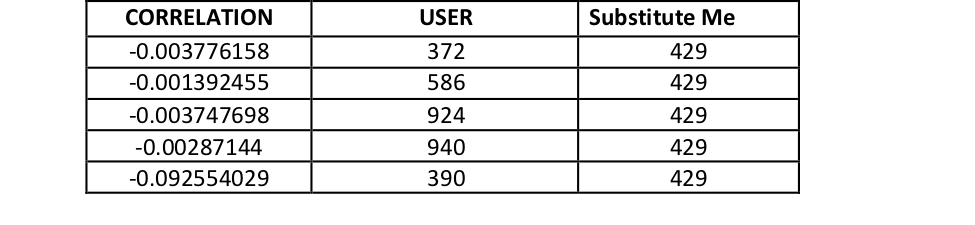
\includegraphics[width=0.6\textwidth]{negativeCorrelation}
      \caption{Negative Correlation}
	\end{figure}
	
\begin{figure}[h]
  \centering
    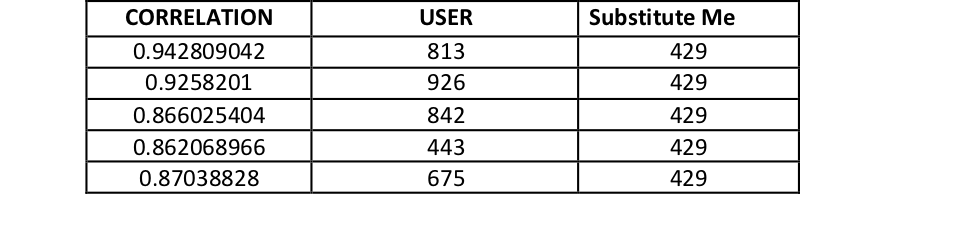
\includegraphics[width=0.6\textwidth]{positiveCorrelation}
      \caption{Positive Correlation}
	\end{figure}

\newpage
 
\end{homeworkProblem}
\clearpage
\newpage

%----------------------------------------------------------------------------------------
%   PROBLEM 3
%----------------------------------------------------------------------------------------

\begin{homeworkProblem}
3.  Compute ratings for all the films that the substitute you have not seen.  Provide a list of the top 5 recommendations for films
that the substitute you should see.  Provide a list of the bottom 5 recommendations (i.e., films the substitute you is almost certain
to hate).\\
%\problemAnswer{

 \textbf{SOLUTION}\\
 
To solve this problem, i have used the code from the text \textbf{Programming Collective Intelligence}
I have used the \textbf{getRecommendations} function to get the recommendations for '\textbf{Substitute Me}.
The results of the same is saved in to a text file \textbf{recommendedMovies.txt}
		      
\begin{lstlisting}[language=Python, caption=recommendation.py]
import csv
import math
import operator
import string
from collections import Counter
from math import sqrt

def sim_distance(prefs, p1, p2):
	'''
	Returns a distance-based similarity score for person1 and person2.
	'''

	# Get the list of shared_items
	si = {}
	for item in prefs[p1]:
		if item in prefs[p2]:
			si[item] = 1
	# If they have no ratings in common, return 0
	if len(si) == 0:
		return 0
	# Add up the squares of all the differences
	sum_of_squares = sum([pow(prefs[p1][item] - prefs[p2][item], 2) for item in
						 prefs[p1] if item in prefs[p2]])
	return 1 / (1 + sqrt(sum_of_squares))


def sim_pearson(prefs, p1, p2):
	'''
	Returns the Pearson correlation coefficient for p1 and p2.
	'''

	# Get the list of mutually rated items
	si = {}
	for item in prefs[p1]:
		if item in prefs[p2]:
			si[item] = 1
	# If they are no ratings in common, return 0
	if len(si) == 0:
		return 0
	# Sum calculations
	n = len(si)
	# Sums of all the preferences
	sum1 = sum([prefs[p1][it] for it in si])
	sum2 = sum([prefs[p2][it] for it in si])
	# Sums of the squares
	sum1Sq = sum([pow(prefs[p1][it], 2) for it in si])
	sum2Sq = sum([pow(prefs[p2][it], 2) for it in si])
	# Sum of the products
	pSum = sum([prefs[p1][it] * prefs[p2][it] for it in si])
	# Calculate r (Pearson score)
	num = pSum - sum1 * sum2 / n
	den = sqrt((sum1Sq - pow(sum1, 2) / n) * (sum2Sq - pow(sum2, 2) / n))
	if den == 0:
		return 0
	r = num / den
	return r


def topMatches(prefs, person, n=5, similarity=sim_pearson,):
	'''
	Returns the best matches for person from the prefs dictionary. 
	Number of results and similarity function are optional params.
	'''

	scores = [(similarity(prefs, person, other), other) for other in prefs
			  if other != person]
	scores.sort()
	scores.reverse()
	return scores[0:n]


def getRecommendations(prefs, person, similarity=sim_pearson):
	'''
	Gets recommendations for a person by using a weighted average
	of every other user's rankings
	'''

	totals = {}
	simSums = {}
	for other in prefs:
	# Don't compare me to myself
		if other == person:
			continue
		sim = similarity(prefs, person, other)
		# Ignore scores of zero or lower
		if sim <= 0:
			continue
		for item in prefs[other]:
			# Only score movies I haven't seen yet
			if item not in prefs[person] or prefs[person][item] == 0:
				# Similarity * Score
				totals.setdefault(item, 0)
				# The final score is calculated by multiplying each item by the
				#   similarity and adding these products together
				totals[item] += prefs[other][item] * sim
				# Sum of similarities
				simSums.setdefault(item, 0)
				simSums[item] += sim
	# Create the normalized list
	rankings = [(total / simSums[item], item) for (item, total) in
				totals.items()]
	# Return the sorted list
	rankings.sort()
	rankings.reverse()
	return rankings


def transformPrefs(prefs):
	'''
	Transform the recommendations into a mapping where persons are described
	with interest scores for a given title e.g. {title: person} instead of
	{person: title}.
	'''

	result = {}
	for person in prefs:
		for item in prefs[person]:
			result.setdefault(item, {})
			# Flip item and person
			result[item][person] = prefs[person][item]
	return result


def calculateSimilarItems(prefs, n=10):
	'''
	Create a dictionary of items showing which other items they are
	most similar to.
	'''

	result = {}
	# Invert the preference matrix to be item-centric
	itemPrefs = transformPrefs(prefs)
	c = 0
	for item in itemPrefs:
		# Status updates for large datasets
		c += 1
		if c % 100 == 0:
			print('%d / %d' % (c, len(itemPrefs)))
		# Find the most similar items to this one
		scores = topMatches(itemPrefs, item, n=n, similarity=sim_distance)
		result[item] = scores
	return result


def getRecommendedItems(prefs, itemMatch, user):
	userRatings = prefs[user]
	scores = {}
	totalSim = {}
	# Loop over items rated by this user
	for (item, rating) in userRatings.items():
		# Loop over items similar to this one
		for (similarity, item2) in itemMatch[item]:
			# Ignore if this user has already rated this item
			if item2 in userRatings:
				continue
			# Weighted sum of rating times similarity
			scores.setdefault(item2, 0)
			scores[item2] += similarity * rating
			# Sum of all the similarities
			totalSim.setdefault(item2, 0)
			totalSim[item2] += similarity
	# Divide each total score by total weighting to get an average
	rankings = [(score / totalSim[item], item) for (item, score) in
				scores.items()]
	# Return the rankings from highest to lowest
	rankings.sort()
	rankings.reverse()
	return rankings


def loadMovieLens():
  # Get movie titles
	movies = {}
	for line in open('item.txt'):
		(id, title) = line.split('|')[0:2]
		movies[id] = title
  # Load data
	prefs = {}
	for line in open('data.txt'):
		(user, movieid, rating, ts) = line.split('\t')
		prefs.setdefault(user, {})
		prefs[user][movies[movieid]] = float(rating)
		print prefs[user][movies[movieid]]
	return prefs

prefs = loadMovieLens()

userId = '429'
r = getRecommendations(prefs, userId) 
f = open("recommendedMovies.txt","w") 
f.write(str(r))
f.close()

\end{lstlisting} 
%}

\newpage
The above code will generate recommendations for \textbf{Substitute Me} in saves in to text file \textbf{recommendedMovies.txt}.

	
\begin{figure}[h]
  \centering
    
\includegraphics[width=0.6\textwidth]{top5Reco}
      \caption{Top 5 Recommended Movies}
	\end{figure}
	
\begin{figure}[h]
  \centering
    
\includegraphics[width=0.6\textwidth]{bottom5Reco}
      \caption{Bottom 5 Recommended Movies}
	\end{figure}

\newpage
 
\end{homeworkProblem}

%----------------------------------------------------------------------------------------
%   PROBLEM 4
%----------------------------------------------------------------------------------------

\begin{homeworkProblem}
4.  Choose your (the real you, not the substitute you) favorite and least favorite film from the data.  For each film, generate a list
of the top 5 most correlated and bottom 5 least correlated films.Based on your knowledge of the resulting films, do you agree with
the results?  In other words, do you personally like / dislike the resulting films?\\

%\problemAnswer{

 \textbf{SOLUTION}\\
 
To solve this problem, i have used the code from the text \textbf{Programming Collective Intelligence}
I have used the \textbf{transformPrefs} function to change the preferences and get the top 5 suggestions from the \textbf{topMatches} function.
The results for my favorite movie \textbf{Star Wars} and my least favorite movie \textbf{Jurassic Park} has been determined with positive and
negative correlations
		      
\begin{lstlisting}[language=Python, caption=movieCorrelation.py]
import csv
import math
import operator
import string
from collections import Counter
from math import sqrt

def sim_distance(prefs, p1, p2):
	'''
	Returns a distance-based similarity score for person1 and person2.
	'''

	# Get the list of shared_items
	si = {}
	for item in prefs[p1]:
		if item in prefs[p2]:
			si[item] = 1
	# If they have no ratings in common, return 0
	if len(si) == 0:
		return 0
	# Add up the squares of all the differences
	sum_of_squares = sum([pow(prefs[p1][item] - prefs[p2][item], 2) for item in
						 prefs[p1] if item in prefs[p2]])
	return 1 / (1 + sqrt(sum_of_squares))


def sim_pearson(prefs, p1, p2):
	'''
	Returns the Pearson correlation coefficient for p1 and p2.
	'''

	# Get the list of mutually rated items
	si = {}
	for item in prefs[p1]:
		if item in prefs[p2]:
			si[item] = 1
	# If they are no ratings in common, return 0
	if len(si) == 0:
		return 0
	# Sum calculations
	n = len(si)
	# Sums of all the preferences
	sum1 = sum([prefs[p1][it] for it in si])
	sum2 = sum([prefs[p2][it] for it in si])
	# Sums of the squares
	sum1Sq = sum([pow(prefs[p1][it], 2) for it in si])
	sum2Sq = sum([pow(prefs[p2][it], 2) for it in si])
	# Sum of the products
	pSum = sum([prefs[p1][it] * prefs[p2][it] for it in si])
	# Calculate r (Pearson score)
	num = pSum - sum1 * sum2 / n
	den = sqrt((sum1Sq - pow(sum1, 2) / n) * (sum2Sq - pow(sum2, 2) / n))
	if den == 0:
		return 0
	r = num / den
	return r


def topMatches(
	prefs,
	person,
	n=5,
	similarity=sim_pearson,
):
	'''
	Returns the best matches for person from the prefs dictionary. 
	Number of results and similarity function are optional params.
	'''

	scores = [(similarity(prefs, person, other), other) for other in prefs
			  if other != person]
	scores.sort()
	# scores.reverse()
	# return scores[0:n]
	lessfavorite = scores[:n]
	favorite = scores[-n:]
	return (lessfavorite, favorite)


def getRecommendations(prefs, person, similarity=sim_pearson):
	'''
	Gets recommendations for a person by using a weighted average
	of every other user's rankings
	'''

	totals = {}
	simSums = {}
	for other in prefs:
	# Don't compare me to myself
		if other == person:
			continue
		sim = similarity(prefs, person, other)
		# Ignore scores of zero or lower
		if sim <= 0:
			continue
		for item in prefs[other]:
			# Only score movies I haven't seen yet
			if item not in prefs[person] or prefs[person][item] == 0:
				# Similarity * Score
				totals.setdefault(item, 0)
				# The final score is calculated by multiplying each item by the
				#   similarity and adding these products together
				totals[item] += prefs[other][item] * sim
				# Sum of similarities
				simSums.setdefault(item, 0)
				simSums[item] += sim
	# Create the normalized list
	rankings = [(total / simSums[item], item) for (item, total) in
				totals.items()]
	# Return the sorted list
	rankings.sort()
	rankings.reverse()
	return rankings


def transformPrefs(prefs):
	'''
	Transform the recommendations into a mapping where persons are described
	with interest scores for a given title e.g. {title: person} instead of
	{person: title}.
	'''

	result = {}
	for person in prefs:
		for item in prefs[person]:
			result.setdefault(item, {})
			# Flip item and person
			result[item][person] = prefs[person][item]
	return result


def calculateSimilarItems(prefs, n=10):
	'''
	Create a dictionary of items showing which other items they are
	most similar to.
	'''

	result = {}
	# Invert the preference matrix to be item-centric
	itemPrefs = transformPrefs(prefs)
	c = 0
	for item in itemPrefs:
		# Status updates for large datasets
		c += 1
		if c % 100 == 0:
			print('%d / %d' % (c, len(itemPrefs)))
		# Find the most similar items to this one
		scores = topMatches(itemPrefs, item, n=n, similarity=sim_distance)
		result[item] = scores
	return result


def getRecommendedItems(prefs, itemMatch, user):
	userRatings = prefs[user]
	scores = {}
	totalSim = {}
	# Loop over items rated by this user
	for (item, rating) in userRatings.items():
		# Loop over items similar to this one
		for (similarity, item2) in itemMatch[item]:
			# Ignore if this user has already rated this item
			if item2 in userRatings:
				continue
			# Weighted sum of rating times similarity
			scores.setdefault(item2, 0)
			scores[item2] += similarity * rating
			# Sum of all the similarities
			totalSim.setdefault(item2, 0)
			totalSim[item2] += similarity
	# Divide each total score by total weighting to get an average
	rankings = [(score / totalSim[item], item) for (item, score) in
				scores.items()]
	# Return the rankings from highest to lowest
	rankings.sort()
	rankings.reverse()
	return rankings

 
def loadMovieLens():
  # Get movie titles
	movies = {}
	for line in open('item.txt'):
		(id, title) = line.split('|')[0:2]
		movies[id] = title
  # Load data
	prefs = {}
	for line in open('data.txt'):
		(user, movieid, rating, ts) = line.split('\t')
		prefs.setdefault(user, {})
		prefs[user][movies[movieid]] = float(rating)
	return prefs

prefs = loadMovieLens()
prefs = transformPrefs(prefs)
(less, high) = topMatches(prefs, 'Star Wars (1977)')
f = open("moviePositiveCorrelation.txt","w") 
f.write(str(less))
f.write('\n')
f.write(str(high))

(less, high) = topMatches(prefs, 'Jurassic Park (1993)')
f = open("moviepNegativeCorrelation.txt","w") 
f.write(str(less))
f.write('\n')
f.write(str(high))
\end{lstlisting} 
%}

The above code will generate top 5 and bottom 5 recommendations for my favorite and least favorite movies and 
are saved in to \textbf{moviePositiveCorrelation.txt} and \textbf{moviepNegativeCorrelation.txt} text files.

	
\begin{figure}[h]
  \centering
    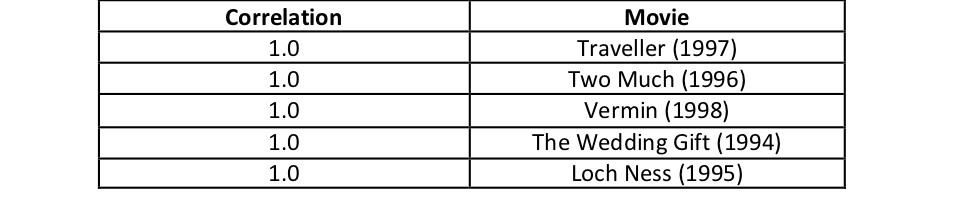
\includegraphics[width=0.6\textwidth]{positive5Favorite}
      \caption{Top 5 Least Favorite Recommendations}
	\end{figure}
	
\begin{figure}[h]
  \centering
    
\includegraphics[width=0.6\textwidth]{negative5Favorite}
      \caption{Bottom 5 Least Favorite Recommendations}
	\end{figure}
	
\begin{figure}[h]
  \centering
    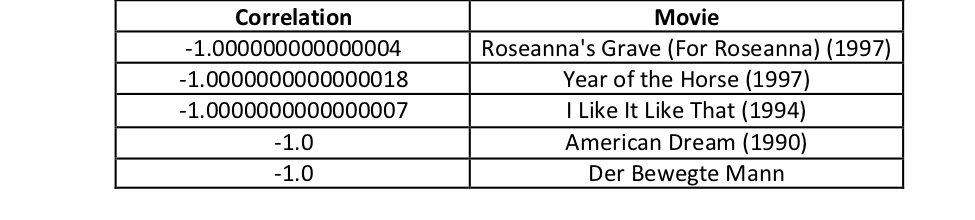
\includegraphics[width=0.5\textwidth]{bottom5fav}
      \caption{Bottom 5  Favorite Recommendations}
	\end{figure} 
	
\begin{figure}[h]
  \centering
    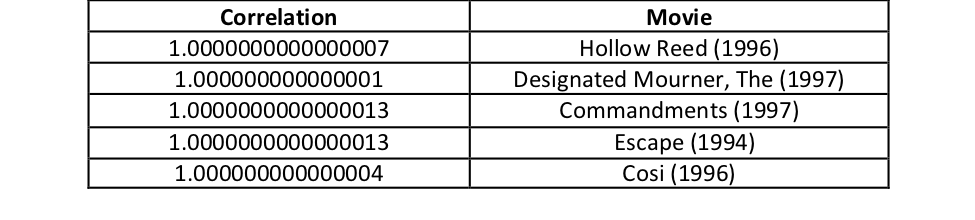
\includegraphics[width=0.6\textwidth]{top5fav}
      \caption{Top 5  Favorite Recommendations}
	\end{figure}
	

	
\end{homeworkProblem}
\newpage
\textbf{References}
\begin{enumerate}
\item\textbf{} https://github.com/arthur-e/Programming-Collective-Intelligence
\item\textbf{} http://grouplens.org/datasets/movielens/100k/
\end{enumerate}
\end{document}
